% CVPR 2024 Paper Template; see https://github.com/cvpr-org/author-kit

\documentclass[10pt,twocolumn,letterpaper]{article}

%%%%%%%%% PAPER TYPE  - PLEASE UPDATE FOR FINAL VERSION
% \usepackage{cvpr}              % To produce the CAMERA-READY version
% \usepackage[review]{cvpr}      % To produce the REVIEW version
\usepackage[pagenumbers]{cvpr} % To force page numbers, e.g. for an arXiv version

% Import additional packages in the preamble file, before hyperref
%
% --- inline annotations
%
\newcommand{\red}[1]{{\color{red}#1}}
\newcommand{\todo}[1]{{\color{red}#1}}
\newcommand{\TODO}[1]{\textbf{\color{red}[TODO: #1]}}
% --- disable by uncommenting  
% \renewcommand{\TODO}[1]{}
% \renewcommand{\todo}[1]{#1}
\usepackage{amsthm}
\usepackage{graphicx}
\usepackage{animate}
\newcommand{\Var}{\textup{Var}}
\newcommand{\Cov}{\textup{Cov}}
\newcommand{\bE}{\mathbb{E}}
\newtheorem{proposition}{Proposition}
\newtheorem{example}{Example}


% It is strongly recommended to use hyperref, especially for the review version.
% hyperref with option pagebackref eases the reviewers' job.
% Please disable hyperref *only* if you encounter grave issues, 
% e.g. with the file validation for the camera-ready version.
%
% If you comment hyperref and then uncomment it, you should delete *.aux before re-running LaTeX.
% (Or just hit 'q' on the first LaTeX run, let it finish, and you should be clear).
\definecolor{cvprblue}{rgb}{0.21,0.49,0.74}
\usepackage[pagebackref,breaklinks,colorlinks,citecolor=cvprblue]{hyperref}

\usepackage{graphicx}
\usepackage{makecell}
\usepackage{hhline}
\usepackage{comment}
% \usepackage{dblfloatfix}

%%%%%%%%% PAPER ID  - PLEASE UPDATE
\def\paperID{} % *** Enter the Paper ID here
\def\confName{CVPR}
\def\confYear{}

\newcommand{\bp}[1]{\textcolor{red}{{[BP: #1]}}}

%%%%%%%%% TITLE - PLEASE UPDATE
\title{Diffusion Illusions: Hiding Images in Plain Sight}

%%%%%%%%% AUTHORS - PLEASE UPDATE
\author{%
\vspace{-0.5em}
  Ryan Burgert \quad
  Xiang Li \quad 
  Abe Leite \quad
  Kanchana Ranasinghe \quad
  Michael S. Ryoo
  \vspace{0.5em} \\
  Stony Brook University \quad 
  \vspace{0.2em} \\
  \small{\texttt{rburgert@cs.stonybrook.edu}}
  \vspace{0.8em} 
}

% \renewcommand{\baselinestretch}{0.98}
\newcommand{\projurl}{\url{https://diffusionillusions.com}}


\begin{document}
% \maketitle


\twocolumn[{%
\renewcommand\twocolumn[1][]{#1}%
    \vspace{-5.8em}
\begin{center}
\maketitle
    \vspace{-2.8em}
    \centering
    % \includegraphics[width=1\textwidth]{figs/TeaserLabeled_Compressed.pdf}
    \includegraphics[width=1\textwidth]{figs/AlignedTeaser_Compressed-crop.pdf}
    \vspace{-1.3em}
    \captionof{figure}{Diffusion Illusions are a new class of automatically generated optical illusions. The images on top demonstrate the three major types of illusions we discuss in this paper: Flip Illusions, Rotation Overlay Illusions, and Hidden Overlay Illusions. (Terminology is formally defined in \cref{sec:problem}). The bottom showcases an example of Hidden Overlay Illusions: four images (prime images $p_{1\dots4}$) that when stacked on top of each other (arrangement) reveal a new fifth image (derived image $d_5$). 
    \textit{Please note that these illustrations are \underline{all photographs} of the generated images \underline{physically fabricated} in the real world.} 
    }
    \label{fig:teaser}
    \vspace{0.5em}
\end{center}%
}]


\begin{abstract}
\vspace{-1.4em}
We explore the problem of computationally generating special `prime' images that produce optical illusions when physically arranged and viewed in a certain way.
First, we propose a formal definition for this problem.
Next, we introduce Diffusion Illusions, the first comprehensive pipeline designed to automatically generate a wide range of these illusions.
Specifically, we both adapt the existing `score distillation loss' and propose a new `dream target loss' to optimize a group of differentially parametrized prime images, using a frozen text-to-image diffusion model.
We study three types of illusions, each where the prime images are arranged in different ways and optimized using the aforementioned losses such that images derived from them align with user-chosen text prompts or images.
We conduct comprehensive experiments on these illusions and verify the effectiveness of our proposed method qualitatively and quantitatively.
Additionally, we showcase the successful physical fabrication of our illusions --- as they are all designed to work in the real world.
Our code and examples are publicly available at our 
\textit{interactive} project website: \projurl
\vspace{-1.5em}
\end{abstract}

\section{Introduction}
An image that is viewed right-side up appears to be an ordinary photo of a dog but viewed upside-down looks like a sloth. Four images, each showing an everyday playground, when superimposed form a QR code (see \cref{fig:teaser}). These types of images that cause illusions have long required immense time and skill to create, but we have developed a general pipeline capable of generating appealing illusions automatically.
More specifically, given a frozen text-to-image diffusion model, we adapt existing score distillation loss and propose a new dream target loss to optimize a group of prime images differentiably parametrized by fourier feature networks.
Eventually, the images are optimized to comply with the textual and/or image prompts given by the user to trigger illusions in a certain arrangement.

Generating such images is not the sole domain of play. Illusions -- that is, visual stimuli whose interpretation depends on how they are arranged and viewed -- have been created and studied for centuries. While they are an appealing sort of ``visual puzzle'', they also reveal much about how humans perceive the world and about the abstract structure of images. Even though illusions have been created and studied for centuries, and certain types have been generated by computers for decades, photorealistic illusions have remained largely out of reach until the very recent past, and until this point, there has been no general framework for understanding and generating such illusions.

\subsection{Contributions}
% \noindent \textbf{Contributions:}
%In this work, we make three main contributions: 
In this paper, we present the first formalized, generic framework for creating such illusions. We name our framework \textit{Diffusion Illusions}. Our major contributions can be summarized as follows:
% The major contributions of this work can be summarized as follows:
\begin{enumerate}[leftmargin=1.5em,noitemsep,topsep=0.0ex,itemsep=-1.0ex,partopsep=0ex,parsep=1ex]
   \item We provide the first formal definition for the problem of generating illusions; 
   \item We present Diffusion Illusions, a flexible tool for generating multiple types of illusions;
   \item We assess the quality of computer-generated illusions in multiple aspects and conduct comprehensive experiments to validate the effectiveness of our method;
   \item We successfully fabricate the generated images and their corresponding illusions in the real world.
\end{enumerate}


\subsection{Related Work: History of Illusions}
\begin{figure}
\centering
\includegraphics[width=1\linewidth]{figs/relatedwork.v3.pdf}
\vspace{-2.0em}
\caption{\small
A brief history of illusions. \textbf{Classical illusions}: (A) ``Fruit Basket'' (1500s) by Giuseppe Arcimboldo provides a very early example, depicting a face when viewed in one orientation and a fruit basket when viewed in the other. (B) When viewed directly, ``Kaninchen und Ente'' (1892) is ambiguous; $45^\circ$ rotations make it appear as a rabbit or a duck \cite{jastrow1899mind, wittgenstein_philosophical_1953}. (C) ``My Wife and My Mother-in-Law'' (1915) by William Ely Hill may be interpreted as showing either a young or an old woman depending on how it is grouped \cite{boring_new_1930, nicholls_perception_2018}. \textbf{Computationally-generated illusions}: (D) a hybrid image which appears to be a leopard when viewed close-up and an elephant when viewed from a distance \cite{oliva2006hybrid}. (E) a wire sculpture which depicts three different 2010s American politicians when viewed from different angles \cite{hsiao_multi-view_2018}. \textbf{Diffusion-based illusions}: (F) an image depicting a duck when viewed upright and a rabbit when rotated $90^\circ$ ccw \cite{tancik_illusiondiffusion_2023}. (G) a set of computationally-generated ambigrams reading `Ohio', `cloud', `yeah', and `python' \cite{samsudin_ambigrams_2023}. (H) an image depicting a giraffe when viewed upright and a penguin when viewed upside-down \cite{geng2023visualanagrams}.}
\label{fig:intro}
\vspace{-1em}
\end{figure}

\subsubsection{Classical illusions}
% \noindent \textbf{Classical Illusions}
Images whose interpretation depends on viewing angle or category bias, sometimes known as ambiguous images, have been designed for centuries. Such images have drawn the scholarly interest of psychologists \cite{jastrow1899mind, boring_new_1930} and philosophers \cite{wittgenstein_philosophical_1953} since the 1800s. Ambiguous images have been used experimentally to understand how category bias during perception varies as people age \cite{nicholls_perception_2018}, and families of ambiguous images, such as ambigrams \cite{hofstadter1985meta}, are often constructed as a way of better understanding the domains they belong to. We present some relevant examples of classical illusions in \Cref{fig:intro}.

\begin{comment}
\begin{figure}
    \centering
    \includegraphics[width=1\linewidth]{mainimage.png}
    \includegraphics[width=1\linewidth]{figs/hidemethod.png}
    \vspace{-2em}
    \caption{Diffusion Illusions are a new class of automatically generated optical illusions. The top image demonstrates our Flip illusion, and the bottom one showcases four transparent images that when stacked on top of each other and put on a backlight reveal fifth images. \textit{Please note that these are all \underline{real photographs}.}}
    \label{fig:teaser}
    \vspace{-2em}
\end{figure}
\end{comment}


\subsubsection{Computationally-generated illusions}
% \textbf{Computationally-generated Illusions} 
A growing stream of research has focused on computationally generating specific types of illusions. One early example is hybrid images \cite{oliva2006hybrid}. Hybrid images are created from two images by combining the low-frequency features of one with the high-frequency features of the other. Viewers see the object from the low-frequency image when viewing the hybrid image from a distance, and see the object from the high-frequency image when viewing up-close. While this process may be automated, the authors note that for best results, the overall shapes of the low-frequency and high-frequency images should be manually aligned.

A number of researchers have created 3-dimensional objects that are interpreted as different objects when they are viewed from different angles. In multi-view wire art \cite{hsiao_multi-view_2018}, a single 3D wire may be viewed or lit from multiple angles to obtain different clean line drawings; and in view-dependent surfaces \cite{perroni-scharf_constructing_2023}, a colored 3D-printed height field may be viewed from different angles to obtain different colored images.

An additional type of illusion is steganography, in which apparently normal objects may be viewed in a particular way to uncover a hidden meaning. In The Magic Lens \cite{papas_magic_2012}, seemingly meaningless dots are generated such that, when viewed through an intricate refractive lens, they will comprise a specified image.




\subsubsection{Diffusion-based Image Generation}
% \noindent \textbf{Diffusion-based Image Generation} 
Diffusion Probabilistic Models \cite{pmlr-v37-sohl-dickstein15} resulted in rapid advances for image generation tasks, including text-to-image generation \cite{Nichol2022GLIDETP,diffusionbeatsgans,dalle,dalle2,imagen,palette,parti,sr3}. Recent works \cite{Poole2022DreamFusionTU,Burgert2022PeekabooTT} sample pre-trained diffusion models without re-training to generate outputs in novel domains. Score Distillation introduced in DreamFusion \cite{Poole2022DreamFusionTU} is the underlying technique enabling optimization of samples in any arbitrary parameter space without backpropagation through the diffusion model. 
We utilize these techniques to construct a novel framework for illusion generation. 
% Recent progress in text-to-image models \cite{} and more specifically text-conditioned diffusion denoising models \cite{} has resulted in the usual boilerplate about impressive generative AI. 
These rapid advances have led to an exploration of suitable evaluation metrics, both quantitative and qualitative \cite{lee_holistic_2023,Benny2020EvaluationMF,Betzalel2022ASO,yeh2023navigating, friedman2022vendi}, which we use to evaluate our proposed framework.

\subsubsection{Contemporary Work}
% \noindent \textbf{Contemporary Work}
Following recent image generation developments, a small but growing body of non-scholarly or unpublished work has approached the problem of generating multi-view 2D images \cite{tancik_illusiondiffusion_2023} or ambigrams \cite{samsudin_ambigrams_2023}. While these approaches appear to yield appealing results, they are narrowly focused on specific illusions, may require substantial cherry-picking, and have not been formally presented or published. 
In contrast, we present a formalized, generic approach capable of generating variable types of illusions followed by extensive evaluation (both quantitative and qualitative) of our approach.
Inspired by our Diffusion Illusions project, contemporary work in \cite{geng2023visualanagrams} presents a formal framework for efficient (fast inference) illusion generation, but operates on a subset of our illusions (namely, those with a single ``prime image'' in our terminology). Furthermore, \cite{geng2023visualanagrams} does not explore any illusions with overlay which is generally more challenging and the generality for real-world transfer (i.e. fabrication of illusions in the real world). 

%%% CONTRIBUTIONS USED TO BE HERE - I MOVED IT UP (ryan)

\section{Problem Statement}
\label{sec:problem}

\begin{figure*}
\centering
% \includegraphics[width=0.7\linewidth]{figs/architecture.v2.pdf}
\includegraphics[width=0.7\linewidth]{figs/architecture.v3.drawio.pdf}
\vspace{-1.0em}
\caption{Architecture overview. Trainable components are shown in blue, intermediate variables are in red, non-trainable functions are in white, and inputs are in green. A diffusion network provides two different loss signals pulling the derived images towards the text prompts. Only a single loss signal, either Score Distillation Loss or Dream Target Loss, is computed at each training step. Gradients on the derived images are backpropagated through the arrangement operations and prime images to the parameters of the Fourier Feature Networks. No backpropagation occurs through the diffusion network.}
\label{fig:overview}
\vspace{-1em}
\end{figure*}
% We define an illusion as the situation that occurs when a set of physically realized \textit{prime} images are \textit{arranged} in multiple ways, each yielding a unique \textit{derived} image representing a specific object or scene. 
We define an illusion as the situation that occurs when a set of physical images called \textit{prime images} $p$ are viewed or \textit{arranged} in multiple ways, with each arrangement yielding a unique perceived image, referred to as a \textit{derived image} $d$, that represents a specific object or scene. 

Most of the existing illusions we have discussed consist of a single 2D image or 3D object as a prime image, with the arrangements being simple translations and rotations of the prime image in 2D or 3D space. In the simplest case where a 2D drawing is rotated to yield different perceived objects, the arrangement operations may be modeled as simple rotations. The near and distant views composing the Hybrid Images illusion \cite{oliva2006hybrid}, on the other hand, might be best modeled by high-pass and low-pass spatial frequency filters.

In an effort to find a fully general definition of illusions and leverage the new possibilities afforded by text-to-image models, we do not limit ourselves to a single prime image. % EXISTING WORK WITH MULTIPLE PRIME IMAGES? Maybe something where multiple things need to align?
We additionally consider situations where \textit{multiple} composable prime images, for instance, stencils or light-filtering transparencies, may be arranged in different ways to yield different derived images. In the particular case of composing two light-filtering transparencies, the arrangement operation may be modeled as a rotation of each prime image followed by a multiply operation to model the light-filtering step.

Formally, the illusion process is described as follows. Consider some prime image space $\mathcal{P}$ representing physically realizable visual stimuli, and some derived image space $\mathcal{D}$ representing a human view of a scene. (Practically, we use 2D RGB images to represent both spaces.) Then, an illusion consists of a tuple of $n$ prime images $\{p_1, p_2, \ldots, p_n\}, p_i \in \mathcal{P}$ and a tuple of $m$ arrangement operations $A = \{a_1, a_2, \ldots, a_m\}, a_j : \mathcal{P}^n \rightarrow \mathcal{D}$. Each $a_j$ represents an arrangement of all of the prime images to obtain a single derived image $d_j$, such that the illusion yields a tuple of $m$ derived images $\{d_1, d_2, \ldots, d_m\}, d_j \in \mathcal{D}$. (This articulation may be easily generalized to heterogeneous illusions, such as a wireframe viewed through a stencil; in this case, each prime image $p_i$ belongs to its own prime image space $\mathcal{P}_i$.)

This framing is complementary to the existing literature on ``ambiguous images''. The illusion process is not intended to cover images that have multiple interpretations when viewed in exactly the same way, though it may be possible to articulate a perceptual bias towards a certain category as a type of arrangement. However, the illusion process otherwise broadens the category of ambiguous images to include situations involving multiple composed images. We propose multiple examples below that are to our knowledge wholly novel.

This definition allows one to separate the process of creating an illusion into two steps: first, selecting a prime image domain and defining and modeling the arrangement operation; and second, searching the prime image domain for images that yield the desired derived images when arranged in each way. While the first step requires creativity and experimentation, the second is sufficiently concrete that it may be practically automated, as discussed in \cref{sec:method}.


% We formally define an illusion as the situation that occurs when at least one physically realized \textit{prime} image may be \textit{viewed} in multiple ways, yielding multiple \textit{derived} images that are perceived as different objects or scenes. Most of the classical illusions we have discussed consist of a single 2D image or 3D object as a prime image, with the views being simple translations and rotations of the prime image in 2D or 3D space. In the simplest case where a 2D drawing is rotated to yield different perceived objects, the prime-to-derived transition may be modeled as a simple rotation. The near and distant views composing the Hybrid Images illusion \cite{}, on the other hand, might be best modeled by high- and low-pass spatial frequency filters.


\section{Method}
\label{sec:method}

We introduce Diffusion Illusions, a flexible tool for generating multiple types of visual illusions that can be styled with unprecedented control (e.g. photorealistic images, artistic styles, or even arbitrary information such as QR codes).
At a high level, the Diffusion Illusions pipeline consists of 
\begin{itemize}[leftmargin=2em,noitemsep,topsep=0.0ex,itemsep=-1.0ex,partopsep=0ex,parsep=1ex]
    \item a set of prime images parameterized by $\theta$ ($\mathcal{P}$),
    \item a set of specific arrangement processes ($A$, that derive images from all primes), 
    \item a frozen text-to-image diffusion model ($\mathcal{F}$)
\end{itemize}
We refer to the outputs of the arrangement processes as derived images ($D$). 
The diffusion model is used to provide a signal using one of two mechanisms (\textit{Score Distillation Loss} or \textit{Dream Target Loss}, which will be covered in \cref{sec:losses}) to suitably optimize the prime images, which in turn modifies the derived images.
Our overall pipeline is illustrated in \cref{fig:overview}.

\subsection{Prime Images}
As described in \cref{sec:problem}, prime images are the physical images we eventually want to generate, that will trigger an illusion when viewed or arranged in multiple ways.

In our framework, prime images are represented as $512 \times 512$ dimensional RGB images, meaning that $\mathcal{P} \simeq \mathbb{R}^{(512,512,3)}$.
Instead of direct pixel-space image representation, we use Fourier Features Networks (FFN)~\cite{tancik2020fourier} to represent prime images in parametric form. 
For each prime image, the learnable weights of a single MLP network act as its representation. 
The MLP network maps image-space coordinates to corresponding RGB values similar to \cite{Burgert2022}, forming an implicit image representation.
We further discuss the advantages of FFN in \cref{sec:discussion}.

% Earlier experiments optimizing prime images directly in pixel space resulted in information being encoded at very high frequencies and requiring pixel-perfect alignment to generate the intended derived images (see \cref{fig:fig-noisy}). While the result was pleasing when viewed digitally, it was impractical for real-world illusions. Motivated by previous arguments \cite{Burgert2022PeekabooTT, Burgert2022}, we elect to use Fourier Features Network \cite{tancik2020fourier} based parametric image representations. 

\subsection{Arrangement Processes}
\label{sec:illusions}
The purpose of arrangement processes, $A$, is to operate on a set of prime images (including single element sets) and produce unique outputs, the derived images. For a single arrangement process $a_i$, 
\begin{align}
    d_i = a_i(P)
\end{align}
each unique sequence of prime images produces a distinct derived image, $d_i$.
Each operation $a_i \in A$ should possess three properties: 
1) For the same set of inputs the operation should always provide the same output (fixed operation). 
2) $a_i$ should also be differentiable, i.e., the possibility to explicitly calculate gradients propagation from output to input through the operation. 
3) $a_i$ should also be realizable in the real world: some series of physical actions on prime images (in physical form) should result in the same derived image. 
To summarize, an arrangement process must be fixed, differentiable, and realizable in the real world. 
\begin{comment}
In our work, we generate illusions belonging to three categories as discussed in \cref{sec:illusions}. 

\begin{itemize}  
\item \textbf{Flip Illusions} utilize two arrangement operations with a single prime image. \todo{describe referring to example figure in intro}
\item \textbf{Rotation Overlay Illusions} utilize 4 arrangement operations with 2 sets of prime images. 
A derived image is obtained by modifying the spatial arrangement of the prime image pair through the rotation of one image relative to the other followed by a multiplicative combination. 
\item \textbf{Hidden Overlay Illusions} utilize 5 arrangement operations on 4 sets of prime images. Four operations select one prime image (identity operation on selected) and the fifth combines all four together (multiplicative). 
\end{itemize}
\end{comment}

% \subsection{Specific Illusions} 
We select three illusion categories for further study:
% we study three types of illusions: a classical illusion \textbf{Flip Illusions}, a minimal expansion to multiple prime images \textbf{Rotation Overlay Illusions}, and an exploration of a complex arrangement combining four prime images \textbf{Hidden Overlay Illusions}.

\begin{itemize}

\item \textbf{Flip Illusion} is one of the most classical types of illusions. We define this illusion as consisting of a single 2D prime image, which is interpreted as some object when viewed upright (the first derived image $d_1$) and as another object when viewed upside-down (the second derived image $d_2$).

\item \textbf{Rotation Overlay Illusion} is a minimal type of illusion involving multiple prime images. This illusion is based on two square light-filtering 2D prime images, one base and one rotator. The rotator image is rotated with 0, 90, 180, and 270 degree angles and superimposed on the base image; each rotation yields a derived image interpreted as a different object (see \cref{fig:rot_illusion}).

\begin{figure}
    \centering
    \includegraphics[width=1\linewidth]{figs/RotationPhoto.pdf}
    \vspace{-2em}
    \caption{This figure shows the rotation overlay illusion arrangement process. \textit{Please note that these are all \underline{real photographs.}} The ``rotator'' image is placed on a ``base'' image over a backlight, both printed out onto transparent sheets. Then, as the rotator spins, we derive four different images. }
    \label{fig:rot_illusion}
    \vspace{-0.5em}
\end{figure}

\item \textbf{Hidden Overlay Illusion} is introduced to push the boundaries of the prime-to-derived relationship, in which four light-filtering prime images, each of which is interpretable on its own, may be merged to obtain a fifth hidden image. Here the modeled view process for the first four derived images is simply the identity function; the view process for the fifth is the product of the four prime images (see \cref{fig:hidden_overlay_animals_photo}).
% The Hidden Overlay Illusion demonstrated in real life. Please note that these are all real photographs.


\end{itemize}
We select these illusion styles to cover varying set cardinalities for prime images and arrangement processes. The arrangement process relevant to each illusion is presented in \cref{tbl:arrangements}. We also present photographs of real-world fabrications for each illusion type in \cref{fig:teaser}, \cref{fig:rot_illusion} and \cref{fig:hidden_overlay_animals_photo}. 
% Note that different illusion styles may involve varying set cardinalities for prime images and arrangement processes. The arrangement process relevant to each illusion is presented in \cref{tbl:arrangements}. 

\begin{figure}
    \centering
    \includegraphics[width=1\linewidth]{figs/overlaydiagram.jpg}
    \caption{This figure shows the rotation overlay illusion arrangement process. \textit{Please note that these are all \underline{real photographs.}}}
    %\caption{\textbf{Hidden Overlay Illusion:} Photographs of different prime images as we overlay them in real life.}
    \label{fig:hidden_overlay_animals_photo}
\end{figure}


\begin{comment}
    


\subsection{Specific illusions}
\label{sec:illusions}
In this paper, we study three types of illusions: a classical illusion, a minimal expansion to multiple prime images, and an exploration of a complex arrangement combining four prime images.

\begin{itemize}

\item The \textbf{Flip Illusion} is one of the most classical types of illusions. We define this illusion as consisting of a single 2D prime image, which is interpreted as some object when viewed upright (derived image 1) and as another object when viewed upside-down (derived image 2).

\item As a minimal type of illusion involving multiple prime images, we introduce the \textbf{Rotation Overlay Illusion}. This illusion is based on two square light-filtering 2D prime images, one base and one rotator. The rotator image is rotated with 0, 90, 180, and 270 degree angles and superimposed on the base image; each rotation yields a derived image interpreted as a different object.

\item In an effort to push the boundaries of the prime-to-derived relationship, we introduce the \textbf{Hidden Overlay Illusion}, in which four light-filtering prime images, each of which is interpretable on its own, may be merged to obtain a fifth hidden image. Here the modeled view process for the first four derived images is simply the identity function; the view process for the fifth is the product of the four prime images.

\end{itemize}

\end{comment}


\begin{table}[t]
\centering
\small
\def\arraystretch{1.8}  % height
\setlength\tabcolsep{0.7em}  % width
\scalebox{0.86}{
\begin{tabular}{cccc}
    \toprule \rowcolor{Gray}
    Illusion & $n$ & $m$ & $\mathbf{a}$ \\ \midrule
    Flip & 1 & 2 & \makecell{$a_1(\mathbf{p}) = p_1$ \\ $a_2(\mathbf{p}) = \mathrm{rot}(p_2, 180)$} \\ \midrule
    Rotation Overlay & 2 & 4 & $a_j(\mathbf{p}) = p_1 * \mathrm{rot}(p_2, 90j)$ \\ \midrule
    Hidden Overlay & 4 & 5 & \makecell{$a_j(\mathbf{p}) = p_j, j \le 4$ \\ $a_5(\mathbf{p}) = p_1 * p_2 * p_3 * p_4$} \\ \bottomrule
\end{tabular}
}
\vspace{-0.5em}
\caption{This table describes our mathematical models of the Flip, Rotation Overlay, and Hidden Overlay illusions, describing the number of prime images $n$, the number of derived images $m$, and the arrangement operator $\mathbf{a}$ mapping from prime image space $\mathcal{P}^n$ to derived image space $\mathcal{D}^m$. The arrangements in the Flip illusion are simply the identity and a 180 degree rotation. The arrangement operations in the Overlay illusions use a multiplication blend operation to model shining light through multiple transparencies; the result is multiplied by a constant and normalized using $\mathrm{tanh}$ to avoid losing dynamic range.}
\label{tbl:arrangements}
\vspace{-0.5em}
\end{table}

%% We can revert back to old format using this if preferred 
% \begin{tabular}{|c|c|c|c|}
%     \hline
%     Illusion & $n$ & $m$ & $\mathbf{a}$ \\
%     \hhline{|=|=|=|=|}
%     Flip & 1 & 2 & \makecell{$a_1(\mathbf{p}) = p_1$ \\ $a_2(\mathbf{p}) = \mathrm{rot}(p_2, 180)$} \\
%     \hline
%     Rotation Overlay & 2 & 4 & $a_j(\mathbf{p}) = \mathrm{tanh}\left(2 * p_1 * \mathrm{rot}(p_2, 90j)\right)$ \\
%     \hline
%     Multiple Overlay & 4 & 5 & \makecell{$a_j(\mathbf{p}) = p_j, j \le 4$ \\ $a_5(\mathbf{p}) = \mathrm{tanh}\left(3 * p_1 * p_2 * p_3 * p_4\right)$} \\
%     \hline
% \end{tabular}

% \subsection{Learning Process}
\subsection{Diffusion Illusion Optimization}
\label{sec:losses}
Having selected three diverse illusion styles, we next discuss the process for learning optimal prime images.
Given fully-differentiable operations (also realizable in the physical world) that arrange a set of prime images to produce a derived image, we leverage two types of losses in successive phases to provide suitable alignment signals to the derived images, which in turn would update the prime images. 
In the first phase, we use \textit{Score Distillation Loss}~\cite{Poole2022DreamFusionTU}, a high-fidelity but expensive algorithm that applies a conditional denoising model to the input at every image update step. 
In the second phase, we introduce the complementary \textit{Dream Target Loss}, a faster technique that pulls the derived images towards periodically updated target images.

Given a frozen text-to-image latent diffusion model $\mathcal{F}$~\cite{rombach2022high} which contains a text encoder $\mathcal{F}_t$, an image encoder $\mathcal{F}_e$ and the denoising network $\mathcal{F}_u$, 
we initialize a series of prime images $p_i$ each represented by a Fourier Feature Network with random parameters $\theta_i$. 
Derived images $d_i$ then can be presented by the arrangement process as introduced in \cref{sec:illusions}.
For each derived image $d_i$, a target $t_i$ that describes in natural language the expected visual appearance of its final form is given by the user. 
% we introduce a target ($t_i$) that describes in natural language the expected visual appearance of its final form. 
% These natural language descriptions $t_i$ are used to control the visual concepts desired in the final derived images. 
% Optionally, one or more $t_i$ can be given as a specific image instead of a text prompt --- letting users hide targets such as QR codes or blocks of text. 
% We will cover such cases at the end of this subsection.
% ; please see the pseudo-code in the appendix for more details. 
% In this paper, $t_i$ is presumed to be a language description unless otherwise specified.

% \noindent
% \textbf{Score Distillation Loss} 
\subsubsection{Score Distillation Loss}
Score Distillation Loss is a widely-used technique to align images with external conditioning such as textual prompts. 
In essence, Score Distillation Loss ($\mathcal{L}^{\text{SD}}$) randomly selects a timestep $\tau$ of the denoising process, adds noise $\eta_\tau$ proportionate to the timestep $\tau$ to a derived image $d_i$ and applies the denoising process, which is conditioned on corresponding $t_i$, to $d_i + \eta_\tau$ to obtain an estimated noise $\hat{\eta_\tau}$. 
The difference, which we implement as a mean absolute error, between the estimated noise $\hat{\eta_\tau}$ and actual noise $\eta_\tau$ provides a signal for the discrepancy between the derived image $d_i$ and the target description $t_i$ for the derived image. 
This difference is normalized by $\tau$ and then provided as a gradient to the derived image and backpropagated through the arrangement process to the prime image. 
Importantly, this process does not require any backpropagation through the diffusion model. 

In summary, as shown in ~\cref{eq:sd_loss}, score distillation loss provides gradients to optimize the image parameterized by $\theta$, such that iterative updates to the image converge its appearance towards the paired text $t_i$. % Minimizing  $\mathcal{L}^{\text{SD}}$ and propagating gradients provide a minimal framework with strong results. 
% We next explore how the compute efficiency of this setup can be improved. 

\begin{align}
    \hat{\eta_\tau} &= \mathcal{F}_u(d_i + \eta_\tau, \tau, \mathcal{F}_t(t_i)) \\
    \mathcal{L}_i^{\text{SD}}(t_i, d_i)&=\| \eta_\tau - \hat{\eta_\tau} \|_1
    \label{eq:sd_loss}
\end{align}

% \subsubsection{Score Distillation Loss}


% one more difference: single step in SDL, fully denoise in Dream Target Loss
% Look at Peekaboo paper.
% Have an image as an input, get gradient for the image.
% Choose a random diffusion timestep, add noise proportional to that timestep. Predict noise at that timestep using U-Net. The gradient is the difference between actual noise and predicted noise. Normalize the gradient based on the timestep.
% Never backpropagate through diffusion network.
% SDL is the start, run this for first iterations -> makes it noisy. Could be omitted.
\subsubsection{Dream Target Loss}
% \noindent
% \textbf{Dream Target Loss} 
Dream Target Loss is a novel optimized version of the Score Distillation Loss for circumstances where it is not trivial for prime image(s) to follow the gradients from the Score Distillation Loss. 
% In a situation where the gradients from multiple derived images are competing to influence the prime images, it is inefficient to apply a full diffusion model at every iteration while this competition is being resolved.

\begin{figure}
  \centering
  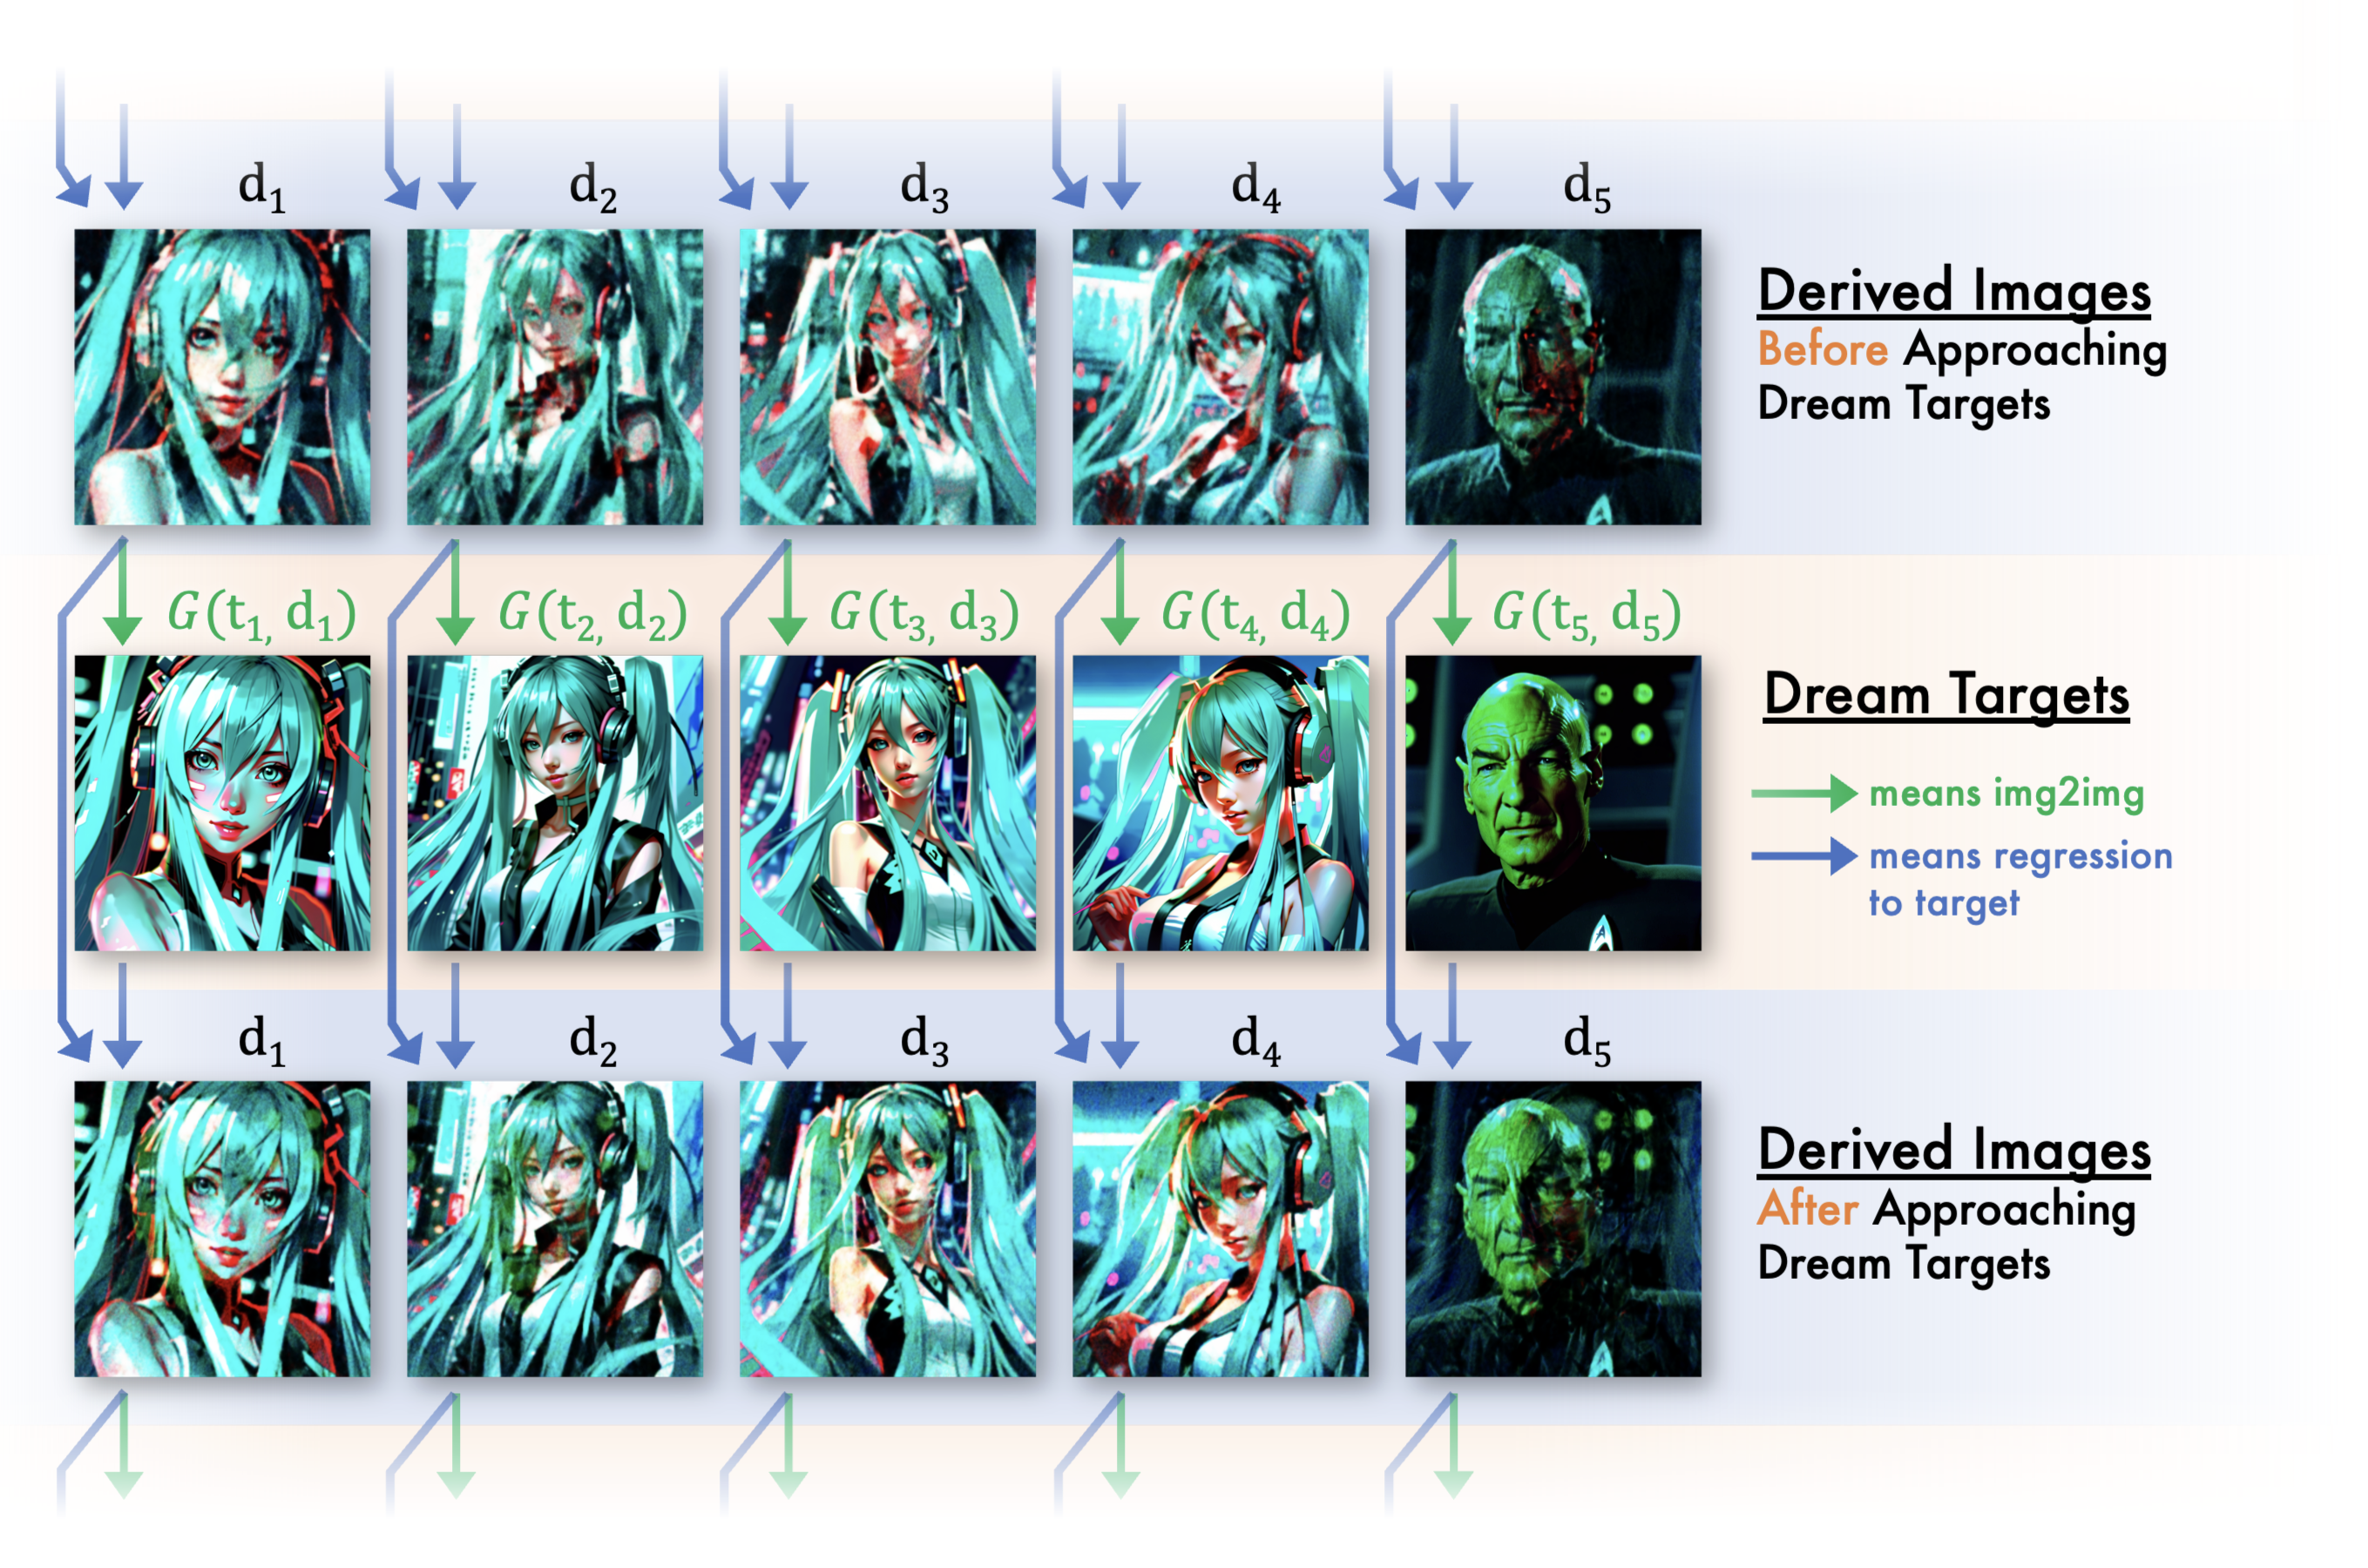
\includegraphics[width=\linewidth, trim={1cm 1cm 6cm 1cm}, clip]{figs/approaching_dreams.png}
  \vspace{-2.0em}
  \caption{We depict the dream-target loss above. It is an iterative process, refining derived images using SDEdit to create target images, which the derived images are then regressed to with gradient descent. Note how the derived images look more like the targets after approaching them than before, such as the man's green face.}
  \label{fig:fig-dream-approach}
  \vspace{-0.5em}
\end{figure}

Instead, Dream Target Loss ($\mathcal{L}^{\text{DT}}$) periodically applies a conditional image-to-image process $z_i = \mathcal{G}(t_i, d_i)$ to obtain a target image $z_i$ for each derived image $d_i$, conditioned on the textual prompt $t_i$.
Then we gradually pull each derived image $d_i$ towards its target image $z_i$ using a combination of the structural image similarity loss ($\mathcal{L}_{SSIM}$) and a pixel-wise mean squared error loss ($\mathcal{L}_{2}$). 

Therein, we obtain a joint loss to similarly learn optimal prime images $p_i$ resulting in derived images aligned to each of our target concepts. 
% \begin{align}
%     \mathcal{L}_i = \mathcal{L}_{SSIM}(\mathcal{G}(t_i), d_i) + \mathcal{L}_{2}(\mathcal{G}(t_i), d_i)
% \end{align}
\begin{align}
    z_i &= \mathcal{G}(t_i, d_i)\\
    \mathcal{L}_i^{\text{DT}}(z_i, d_i) &= \mathcal{L}_{\text{SSIM}}(z_i, d_i) + \mathcal{L}_{2}(z_i, d_i)
    \label{eq:img_sim}
\end{align}

% In the case that $t_i$ is given as an image instead of a text prompt, we instead set $z_i = t_i$ --- useful for when we want to target a specific image such as a QR code.


An additional feature of the Dream Target Loss relative to the SD variant is that it tends to introduce less noise. 

The total dream target loss is a weighted average across all per derived image loss terms.
% , $\mathcal{L}_i^{\text{DT}}$ to obtain, 
\begin{align}
    \mathcal{L}^{\text{DT}} = \sum w_i \mathcal{L}_i^{\text{DT}}
\end{align} where the loss terms are weighted by importance values $w_{1\dots m}$. By default, all $w_i=1$ except in the hidden overlay illusion where the hidden image is prioritized via $w_5=3$.

In practice, for each target image, we optimize the prime image for multiple (i.e. $1000$) steps using the dream target loss. 
Then we repeat the process with the latest prime image so that the target image is updated towards the current derived image for faster convergence (Illustrated in \cref{fig:fig-dream-approach}). 
We implement $\mathcal{G}$ using SDEdit~\cite{meng2022sdedit} where random noise is first added to the input image, and the noisy image is then iteratively denoised conditioned on the text prompt using a frozen diffusion model to generate an output image (see \cref{sec:pseudocode}). 
% We define new image targets as $z_i = \mathcal{G}(t_i, d_i)$ for each derived image using the same textual targets, 

Note that in both Score Distillation Loss and Dream Target Loss, we propagate gradients to the prime images, updating their parametric representation (i.e. the weights of the MLP Fourier Feature Networks $\theta$), and the diffusion model is kept frozen.

% \noindent
% \textbf{Visual Prompt} 
\subsubsection{Visual Prompt}
Optionally, one or more $t_i$ can be given as a specific target image instead of a text prompt --- letting users hide targets such as QR codes or blocks of text. 
In that case, for both phases, the discrepancy between the derived image and the target image is measured using \cref{eq:img_sim}, providing gradients for the prime images.

\subsection{Fabrication}
The flip illusions are trivial to manufacture in real life and need only a printer. The hidden overlay and rotation overlay illusions are created by printing their prime images on overhead display sheets on a color laser printer, before being laminated to protect them from scratches.  % It's a really simple process! 
With a strong enough backlight, the hidden overlays and rotation overlay illusions can be performed on regular pieces of paper as well.

% (Provide examples of target derived image update process, with different image-to-image weights.)


% \subsection{Optimization Schedule}





\section{Experiments}
In this section, we evaluate our framework presenting qualitative visualizations and quantitative metrics. % We focus on the three styles of illusions presented in \cref{sec:illusions} for all evaluations. 

\subsection{Qualitative Evaluation}
We illustrate randomly selected example outputs of our Diffusion Illusions framework. Visualizations for our three selected illusion styles, Flip Illusion, Rotation Overlay Illusion, and Hidden Overlay Illusion are presented in \cref{fig:galflip},
\cref{fig:galrot}, and \cref{fig:galhid} respectively. 
% are shown in \cref{fig:galflip}, Hidden Overlay Illusions are shown in \cref{fig:galhid}, and Rotation Overlay Illusions are shown in \cref{fig:galrot}.
For more interactive examples, please refer to the project website \projurl

\begin{figure}
    \centering
    % \includegraphics[width=.8\linewidth]{figs/FlipGallery.pdf}
    \includegraphics[width=.7\linewidth, trim={0 0 0 1cm}, clip]{figs/rearrangeFlipIllusion.pdf}
    \vspace{-0.5em}
    \caption{\textbf{Flip Illusion Examples:} Please view these images upside-down as well as right-side-up to see two different subjects.  Note: In this illusion,  $d_1 = p_1$}
    % \textit{Please zoom in!}  
    \label{fig:galflip}
    \vspace{-0.5em}
\end{figure}

\begin{figure}
    \centering
    % \includegraphics[width=0.7\linewidth]{Gallery2.png}
    % \includegraphics[width=1\linewidth]{figs/FixedRotationFigure.pdf}
    % \includegraphics[width=1\linewidth]{figs/lessRotationOverlay.pdf}
    % \includegraphics[width=1\linewidth,trim={0cm 1cm 1cm 0cm}, clip]{figs/rearrangeRotationIllusion.pdf}
    \includegraphics[width=0.98\linewidth,trim={0cm 0cm 1cm 0cm}, clip]{figs/rotGal.pdf}
    \vspace{-0.5em}
    \caption{\textbf{Rotation Overlay Examples:}  On the left are the two prime images $p_1$, $p_2$, and on the right are the four derived images $d_{1\dots 4}$ that are obtained by taking the product of the primes, simulation of them overlaid on a backlight.}
    \vspace{-0.5em}
    % \textit{Please zoom in!} 
    \label{fig:galrot}
\end{figure}

\begin{figure}
    \centering
    \includegraphics[width=0.96\linewidth, trim={0 0.95cm 0 0}, clip]{figs/hiddenGal.pdf}
    % \includegraphics[width=1\linewidth]{figs/GalHid.pdf}
    %\includegraphics[width=1\linewidth]{figs/HiddenOverlayGallery.pdf}
    % \centering\includegraphics[width=1\linewidth]{figs/rearrangeHiddenOverlay.pdf}%\includegraphics[width=1\linewidth]{figs/HiddenOverlayGallery.pdf}
    \vspace{-0.5em}
    \caption{\textbf{Hidden Overlay Examples:} On the left are the four prime images $p_1$, $p_2$, $p_3$, $p_4$ and on the right is the derived image $d_5 = p_1 \cdot p_2 \cdot p_3 \cdot p_4$, which simulates overlaying them over a backlight. Note: In this illusion,  $d_i = p_i$ for $i\in 1\dots 4$}
    \vspace{-0.5em}
    \label{fig:galhid}
    % \textit{Please zoom in!}  
\end{figure}






% \todo{xl: please specify the model and the algorithm used to generate the cherry-pick sample
% qualitative images, grid stuff

% 1. Regular samples;  along with the clip score heatmap

% 2. QR code

% 3. Text 

% 4. we can do more like rotation and it will appear in appendix
% }
\subsection{Quantitative Evaluation}
\label{sec:numbers}
Next, we quantitatively benchmark the Hidden Overlay Illusion generated by the variants of Diffusion Illusion in multiple aspects and demonstrate the generalization ability and robustness of the proposed framework. Please check  Appendix~\ref{sec:more_eval} as well for other illusions and more details.

\noindent\textbf{Image Generation Protocol} \quad We design a pipeline that constructs diverse textual prompts randomly and automatically. 
The pipeline relies on two sets of textual prompts. 
The first set $T^s$ is of sentences where each sentence describes a unique art style of an image and contains one \textit{subject} token representing the potential subject of the sentence. 
The second set $T^o$ is of different subjects like `dog', `cat', `car', and so on.
When generating images with a specific style $t^s \in T^s$, we uniformly sample five unique subjects $t^o_i$ where $i \in\{1, \ldots, 5\}$ from $T^o$.
Then we substitute the \textit{subject} token in $t^s$ with $t^o_i$ to construct the textual prompt $t_i$.
Finally, $t_1, \ldots, t_5$ is used to guide the generation of derived images.

For a full evaluation, the whole pipeline is repeated for $N$ times per style $t^s$ to generate $N$ groups of illusion images.
In practice, we set $|T^s| = 4$, $T_o$ is the set of all object classes except `person' in PASCAL VOC~\cite{everingham2010pascal} ($|T^o|=19$), and $N=64$. % [xl: number by average, not true!]. 
Please refer to the Appendix~\ref{sec:more_eval} for the complete list of subjects and styles.

\noindent\textbf{Evaluation Metrics} \quad Inspired by recent works on diffusion model evaluation~\cite{yeh2023navigating, lee2023holistic}, we measure the following properties of the derived images:

\begin{itemize}
    \item \textit{Controllability:} how well the generated images align with the textual prompts. For each generated image and its corresponding textual prompt, we measure the \textit{average cosine similarity} between the image embedding and the text embedding, extracted from a pretrained CLIP~\cite{radford2021learning} model.
    \item \textit{Diversity:} the variety of generated images conditioned on the same prompt. For images generated by the same textual prompt, we calculate two \textit{Venti scores}~\cite{friedman2022vendi} independently based on two visual embeddings: the \texttt{[CLS]} embeddings of DINOv2~\cite{oquab2023dinov2} and CLIP visual embeddings (see Appendix). % and DINOv2+reg~\cite{darcet2023vision}.
    \item \textit{Aesthetics:} the assessment of an image's visual appeal and artistic quality. For each image, we utilize AVA LAION-Aesthetics Predictor V2, which is pretrained on AVA~\cite{murray2012ava} dataset, to estimate an aesthetics score range from 0 to 10. 
    % In addition, we collect a score from GPT-4 Turbo with vision~\cite{openai2023gpt4} using a predefined prompt to reflect the image quality (see Appendix).
    % In addition, we collect a score from a vision language model LLaVA-1.5~\cite{liu2023visual, liu2023improved} using a predefined prompt to reflect the image quality (see Appendix).
    
\end{itemize}

In addition, we study a new property ~\textit{Independence} specifically for the illusion scenario. 
Intuitively, each image is expected to stick to its corresponding textual prompt while not being distracted by other textual prompts in the same group.
Such property is named as \textit{Independence}, which is different from \textit{Controllability} because independence is designed to reflect not only the similarity between an image and its corresponding textual prompt but also the \textit{dissimilarity} between the image and the textual prompts for other images. 
In other words, this property focuses on how well the prime images can `hide' the overlay image or how challenging it will be for people to infer the overlay image from a single prime image and vice versa. 

\begin{itemize}
\item \emph{Independence Score:} Therefore, we propose a new metric Independence Score to reflect such property. Consider a set of $m$ derived images, denoted as $\{d_1, d_2, \ldots, d_m\}$, along with their corresponding textual prompts $\{t_1, t_2, \ldots, t_m\}$. Initially, we extract the visual embeddings $v_i=f_v(d_i)$ and text embeddings $e_j=f_t(t_j)$ using the visual encoder $f_v$ and the text encoder $f_t$ from a pretrained CLIP~\cite{radford2021learning} model respectively. Subsequently, we compute the cosine similarity $k_{ij}=\text{CosineSimilarity}(v_i, e_j)$ between any visual and text embeddings $v_i$ and $e_j$. The results are assembled into a matrix $K$, where $k_{ij}$ is put in the $i$-th row and $j$-th column. The Independence Score $S_\mathrm{IS}$ is calculated by the following equations.
\begin{align}
% \label{eq:inscore}
K_0 &= \mathrm{Softmax}(K / \tau, 0) \\ 
K_1 &= \mathrm{Softmax}(K / \tau, 1) \\ 
S_\mathrm{IS} & := \min(\mathrm{diag}(K_0) \cup \mathrm{diag}(K_1)) 
\end{align}
where $\tau=0.05$ is a temperature constant, $\text{Softmax}(\cdot, l)$ stands for softmax operation along $l$-th dimension and $\text{diag}(\cdot)$ presents a set of the diagonal elements of $(\cdot)$. 
$S_\mathrm{IS}$ is designed to become higher when all images $d_i$ align best with their corresponding textual prompts compared with other textual prompts.
\end{itemize}

\noindent\textbf{Methods} \quad The baseline method of our experiments is a vanilla SDXL generating target images with corresponding textual prompts independently for one step using score distillation loss. We benchmark four variants of our methods named A, B, C, and D. Method C is our default method. It involves 500 steps of score distillation loss followed by 8 steps of dream target loss and applies relative weights [1,1,1,1,3] respectively - which prioritizes the quality-derived hidden image over its constituent primes. In addition, Method A uses Stable Diffusion 1.5 instead of SDXL, which is used by all other methods. Method B uses equal weights for all derived images, using weights [1,1,1,1,1] respectively. Lastly, method D uses 4000 steps of score distillation loss followed by 1 step of dream target loss for smoothness, to evaluate the ability of score distillation loss alone in this task.
% - which we found sometimes lets the fifth image, D5, collapse to black - resulting in lower scores on our metrics.
For fairness, all methods were constrained to run in a 15-minute time window on a single NVIDIA A100 GPU.

\noindent\textbf{Results} \quad For all metrics, we report the score distributions achieved by our default method and the baseline in \cref{fig:big-baseline-fig}. 
\begin{figure}[h]
  \centering
  \includegraphics[width=1\linewidth]{figs/fig-overall-baseline.pdf}
  \vspace{-0.5em}
  \caption{Comparison of multiple score distributions. Refer to axes for metrics. Our framework clearly outperforms the baseline for all metrics except diversity (Vendi Score). We argue the additional constraints intrinsic to our task (of generating illusions) contributed to reduced diversity.}
  \label{fig:big-baseline-fig}
\end{figure}

Our method significantly outperforms the baseline in all metrics except the Vendi Score, which is expected because, for our method, there are more constraints from the derived images applied during the generation process.

The score distributions of four variants of our method are presented in \cref{fig:big-score-fig}. Each row of \cref{fig:big-score-fig} presents two metrics. The subfigures on the left-hand side show the overall performance of a specific method. 
In general, all methods perform similarly well in terms of Controllability (Cosine Similarity) and Diversity (Vendi Score) (the first two rows in \cref{fig:big-score-fig}). Method C shows significant advantages in Aesthetics (Aesthetics Score) and Methods C and D achieve relatively higher Independence Score. 

\begin{figure}[h]
  \centering
  \includegraphics[width=\linewidth]{figs/final-clip_score.png}
  \includegraphics[width=\linewidth]{figs/final-vendi_score_dino.png}
  \includegraphics[width=\linewidth]{figs/final-aesthetics_score.png}
  \includegraphics[width=\linewidth]{figs/final-rm.png}
  \vspace{-0.5em}
  \caption{Score distributions over methods (left) and styles (right). A, B, C, D stands for four variants of our method. Results indicate the significance of prompts for illusion generation.}
  \label{fig:big-score-fig}
\end{figure}


A detailed look at different art styles is presented on the right-hand side of each row of \cref{fig:big-score-fig}, where different metrics respond diversely to different art styles.
Controllability (Cosine Similarity) prefers Style 3 and Style 4 while the Diversity (Vendi Score) prefers Style 2. 
The Aesthetics Score and Independence Score are generally robust to the different styles.
However, the Aesthetics Score prefers Style 4 slightly more than Style 1.

In conclusion, the prompts used are far more important than the chosen implementation. There is no clear one-size-fits-all method indicated by our quantitative evaluations, however, we observe that depending on the art styles and subjects used, a different method will be optimal. 
% than they are to the method variants.
One should carefully pick up a method when generating illusions in a specific art style.
% In conclusion, there is no clear winner given all the quantitative evaluations, and we observe that different metrics are more sensitive to the art styles instead of the variants of methods.
% One should carefully pick up a method when generating illusions in a specific art style.
A further study on subjects is available in the Appendix.

\subsection{Discussions}
\label{sec:discussion}
In this section, we discuss several observations that may inspire future investigation.

\noindent\textit{Q1: Can Diffusion Illusion yield better images when running for a longer time?} 

\noindent Yes. \cref{fig:fig-grad-increase} presents the trend of Controllability (Cosine Similarity) and Aesthetics (Aesthetics Score) as the images used in \cref{sec:numbers} are getting optimized. 
% The relative time indicates the wall clock time passed for optimization, where 0 means the beginning of the optimization and 1 means the end of the optimization. 
% For all four methods, there is a significant trend that all scores increase as the training goes on.
The term `relative time' is employed to denote the progression of wall-clock time during the optimization process. 
A relative time value of 0 means the beginning of optimization, whereas a value of 1 marks its conclusion. 
\cref{fig:fig-grad-increase} reveals a notable trend: there is a consistent increase in metrics as the optimization process advances.
\begin{figure}[h]
  \centering
  \includegraphics[width=0.4\textwidth]{figs/final-grad.png}
  \caption{CLIP Cosine Similarity (left) and Aesthetics Score (right) increase when optimizing for a longer time.}
  \label{fig:fig-grad-increase}
\end{figure}

\noindent\textit{Q2: Is Independence Score a qualitatively valid metric?}

\noindent Generally yes. \cref{fig:fig-sis} shows four illusions randomly selected with diverse independence scores. For each row, the subject of each image is listed above, and the method, style, and independence scores are listed on the left-hand side. 
The four images grouped in the middle are prime images and they derive the overlay image on the right-hand side.
For the first two examples where the independence score is relatively high, each image aligns with its corresponding textual prompt. 
However, for the third example, the overlay image is not closely related to the subject `sofa', resulting in a lower independence score. 
Furthermore, in the last example of \cref{fig:fig-sis}, the overlay image visually biases more towards `cow' instead of `bottle', leading to the lowest independence score.

\begin{figure}[h]
  \centering
  \includegraphics[width=\linewidth]{figs/sis_large_demo.jpg}
  \caption{Examples with diverse independence scores}
  \label{fig:fig-sis}
\end{figure}

\noindent\textit{Q3: What are the reasons to use Fourier Features Network?} 

\noindent Earlier experiments optimizing prime images directly in pixel space resulted in information being encoded at very high frequencies and requiring pixel-perfect alignment to generate the intended derived images (see \cref{fig:fig-noisy}). While the result was pleasing when viewed digitally, it was impractical for real-world illusions. Motivated by previous arguments \cite{Burgert2022PeekabooTT, Burgert2022}, we elect to use Fourier Features Network \cite{tancik2020fourier} based parametric image representations. 

\begin{figure}[h]
  \centering
  \includegraphics[width=\linewidth]{figs/demo_noisy_fft.jpg}
  \caption{A Hidden Overlay image with prime images optimized directly in pixel space. While high-frequency encoding of the hidden image results in less perceivable interference in each individual image, it results in a brittle illusion that is disrupted without pixel-perfect printing and alignment.}
  \label{fig:fig-noisy}
\end{figure}



% \subsection{Comparison to Related Work}
% \subsubsection{Summary}

% 1. different methods are good at different aspects, overall it works

% 2. if you keep training, you will get better results

% 3. the current metrics suck, prompt matters more

% more on appendix

% \subsection{Discussion}

\section{Conclusion}
In this paper, we establish the formal definition of the problem of generating illusions and introduce Diffusion Illusions, a versatile pipeline designed for the generation of a diverse array of illusions. 
Complemented by comprehensive experiments conducted across multiple facets, we verify the effectiveness of our proposed method qualitatively and quantitatively.
We also successfully fabricate the prime images in the real world.
% \todo{xl: I'm going to add some future works}
% In addition, we observe that in some cases, the arrangement of Hidden Overlay Illusion in \cref{tbl:arrangements} may not precisely reflect the actual overlay arrangement when the prime images are printed out. Even the inconsistent performance of different printers may compromise the performance (see Appendix).
% We hope this paper and the issues above inspire further study on more types of illusion generation and creative ways to take advantage of diffusion models. 
Other areas to explore include more types of illusion generation and creative ways to take advantage of diffusion models. 

\vspace{2em}
\noindent
\textbf{Limitations}  \quad
The main limitation of our framework is the relatively high inference time required for generating illusions. While our framework improves over plain score distillation in terms of inference time, we are still slow. Improving the speed of illusion generation frameworks such as ours presents an interesting future direction. 
We note that contemporary work has already explored ways to minimize this inference time. 

Furthermore, 
% the accuracy of the Rotation Overlay or Hidden Overlay illusions might vary due to physical imperfections in the printing process - leaving room for further exploration. 
the effectiveness of visual illusion in the real world may vary a lot due to the errors introduced in the printing process. \cref{fig:simreal2} and \cref{fig:simreal} present the effect of the color shifts when printing the images.

\begin{figure}[t]
  \centering
  % \includegraphics[width=1\linewidth]{figs/simreal2.png}
  \includegraphics[width=1\linewidth, trim={1cm 1cm 1cm 1cm}, clip]{figs/SimRealRot.jpg}
  \caption{The colors shift after printing out Rotation Overlay Illusion images. First row: digital copy of the images and the overlay simulation. Second row: real-world photos of the printed images.}
  \label{fig:simreal2}
\end{figure}

\begin{figure}[t]
  \centering
  \includegraphics[width=1\linewidth]{figs/SimRealHidAdjust.jpg}
  \caption{The colors shift after printing out Hidden Overlay Illusion images. First row: digital copy of the images and the overlay simulation. Second row: real-world photos of the printed images.}
  \label{fig:simreal}
\end{figure}

Other limitations include biases contained in our models (discussed in detail under the ethics statement). 

\vspace{1em}
\noindent
\textbf{Reproducibility Statement}  \quad
Our work builds off open-source models whose pre-trained weights are publicly available. Our framework simply performs inference time optimizations to generate illusions. In our paper, we detail all specifics of our implementation (including PyTorch style pseudo-code) necessary to generate such illusions. Our code (and all material necessary to replicate results in paper) will be released publicly. 

\vspace{1em}
\noindent
\textbf{Ethics Statement}  \quad
A main ethical concern for any generative art model is that it will reduce the demand for human artists in its domain. Generating optical illusion artwork is a very difficult artistic task, and there are few artists that attempt it. Thus, the genre of illusions is currently relatively small and there is limited demand for illusions at present. Diffusion Illusions makes the generation of optical illusions accessible to the general public, making illusions more accessible to the layperson. We believe that, if anything, Diffusion Illusions and related works are likely to increase interest in illusions and the demand for human-created illusions as a result.
Secondly, our experiments utilize Stable Diffusion 1.5 and Stable Diffusion-XL models, and thus our reference implementation of the Diffusion Illusions pipeline will replicate any biases contained within these models. These models are trained on the LAION-2B(en) and LAION-5B datasets, and may over-represent English-language or Western content. The Stable Diffusion 1.5 and Stable Diffusion-XL models are intended for research purposes only, and thus our reference implementation should also be used exclusively for research and informative purposes. Some recent models, including DeepFloyd, are licensed for limited production use and our pipeline easily generalizes to them; however, they have higher system requirements.

\vspace{1em}
\noindent
\textbf{Contributions}  \quad
RB led the project, conceived the prime image / derived image illusion relationship, invented the classes of hidden and rotation overlay illusions, and designed \& implemented the Diffusion Illusions pipeline.
XL designed and performed all quantitative evaluation experiments.
AL formalized and wrote the Illusion problem statement and contributed to paper writing.
KR discussed multiple aspects of the project, supported designing a prior framework (Peekaboo~\cite{Burgert2022PeekabooTT}) important for building our setup, and contributed to paper writing.
MR supervised the project, advised on research direction, and discussed all aspects of the project.  

\vspace{1em}
\noindent \textbf{Acknowledgements} \quad
We would like to thank Brian Price and Jinghuan Shang for helpful discussions about this paper, and Jongwoo Park for both his discussions as well as posing for the flip illusion photo in \cref{fig:teaser}. This material is based upon work supported by the National Science Foundation Graduate Research Fellowship under Grant No. 2234683.


% \clearpage
% \newpage

{
    \small
    \bibliographystyle{ieeenat_fullname}
    \bibliography{main}
}

% WARNING: do not forget to delete the supplementary pages from your submission 
\clearpage
%\setcounter{page}{1}
\maketitlesupplementary

\section{Gaussianity preservation of our noise warping algorithm}

In this section, we discuss our noise warping algorithm, providing a formal proof of its Gaussianity preservation properties. We also present an illustrative example that demonstrates how noise that undergoes expansion and subsequent contraction returns to its original state, showcasing how our noise warping algorithm maintains the underlying Gaussian distribution throughout the warping process.

\begin{proof}
    For each $(x,y) \in V$, $R(x,y)$ is a collection of upsampled noise $X_i$, where
    \begin{align*}
    \bE[X_i] &= \bE[\frac{q(x,y)}{d}] + \bE[\frac{1}{\sqrt{d}}(Z_i - \frac{S}{d})] = 0  \\
        \Var(X_i) &= \Var(\frac{q(x,y)}{d}) + \Var(\frac{1}{\sqrt{d}}(Z_i - \frac{S}{d})) \\
        &= \frac{1}{d^2} + \frac{1}{d} \Var(\frac{d-1}{d}Z_i - \sum_{j\neq i} \frac{Z_j}{d}) \\
        &= \frac{1}{d^2} + \frac{1}{d} \frac{(d-1)^2 + (d-1)}{d^2} = \frac{1}{d},
    \end{align*}
    where we used the fact that $q(x,y)$ and $Z_i$'s are i.i.d. standard Gaussians.
    Since $X_i$ is constructed as a weighted sum of Gaussians, itself is also a Gaussian.
    Moreover, for $i \neq j$, we compute
    \begin{align*}
        &\Cov(X_i, X_j) \\
        =&\Cov(\frac{q(x,y)}{d} + \frac{1}{\sqrt{d}}(Z_i - \frac{S}{d}), \frac{q(x,y)}{d} + \frac{1}{\sqrt{d}}(Z_j - \frac{S}{d})) \\
        =& \frac{1}{d^2} + \frac{1}{d}\bE[(Z_i - \frac{S}{d})(Z_j - \frac{S}{d})] \\
        =& \frac{1}{d^2} + \frac{1}{d}(0 - 2 \frac{\bE[Z_i S]}{d} + \frac{\bE[S^2]}{d^2}) \\
        =& \frac{1}{d^2} + \frac{1}{d}(-\frac{2}{d} + \frac{1}{d}) = 0.
    \end{align*}
    Hence all $X_i$'s are independent.

    For each $(x',y') \in V'$, if $\deg_G((x',y')) = 0$, then $q'(x',y')$ is sampled as an independent standard Gaussian. 
    Otherwise, the output noise pixel $q'(x',y')$ is built as a weighted sum of $R(x,y)\text{.pop}()$ for each edge $((x,y), (x',y'))\in E$, where $R(x,y)\text{.pop}()$ is an independent Gaussian of mean 0 and variance $\frac{1}{\deg_G((x,y))}$.
    Hence $q'(x',y')$ is also a Gaussian with mean 0.
    The variable $s$ after executing the inner for loop thus represents the variance of $q'(x',y')$, so the renormalization at the end brings $q'(x',y')$ back to a standard Gaussian.
    Since the composing $X_i$'s are independent, the resulting noise $q'$ should also have an independent Gaussian in each pixel.
\end{proof}

\begin{example}[Exact recovery of \expansion-\contraction]
Consider the following evolution of noise across three frames with forward flows $f_{i\to j}$ going from frame $i$ to frame $j$ with $i + 1 = j$ (and backward flow if $i -1 = j$).
Suppose at frame $1$, a pixel $v \in D$ with density $1$ has noise $q$. Suppose further that $v'_a$ is a pixel at frame $2$ such that $f_{1\to 2}^{-1}(v'_a) = \{v\}$, and $v'_b \in D$ is the only pixel at frame $2$ such that $f_{1\to 2}^{-1}(v_b') = \varnothing$ and $f_{2\to 1}(v'_b) = v$.
This represents the scenario where $v$ is expanded into two pixels $v'_a,v'_b$.
Then \cref{alg:main} with forward flow $f_{1\to 2}$ and backward flow $f_{2 \to 1}$ will result in $v'_a$ having density $1/2$ and noise $\frac{q}{2} + \frac{1}{\sqrt{2}}(\frac{Z_a-Z_b}{2})$, and $v_b'$ having density $1/2$ and noise $\frac{q}{2} + \frac{1}{\sqrt{2}}(\frac{Z_b-Z_a}{2})$, where $Z_a$ and $Z_b$ are i.i.d. standard Gaussians.
Now, from frame $2$ to frame $3$, suppose there exists a pixel $v''$ such that $f_{2\to 3}^{-1}(v'') = \{v'_a,v'_b\}$, i.e., they both $v'_a$ and $v'_b$ contract to $v''$, and that $f_{3\to2}(D) \cap \{v'_a,v'_b\} = \varnothing$.
Then \cref{alg:main} with forward flow $f_{2\to 3}$ and backward flow $f_{3\to 2}$ will result in $v''$ having density $1$ and noise $q$, hence deterministically recovering the noise and density of $v$ in frame 0.

\end{example}


\section{Qualitative results of training-free image diffusion based video editing}

Noise warping methods that do not preserve Gaussianity degrade per-frame performance, as originally pointed out in~\cite{chang2024warped}. For example, using nearest neighbor and bilinear interpolation destroys the Gaussianity (see \cref{fig:supp_warped_noise_flow_vis}) and consequently deteriorates the per-frame performance on pre-trained image-to-image diffusion models (see \cref{fig:supp_davis_deepfloyd} and \cref{fig:supp_diffrelight_noisewarp}).

\begin{figure*}
    \centering
    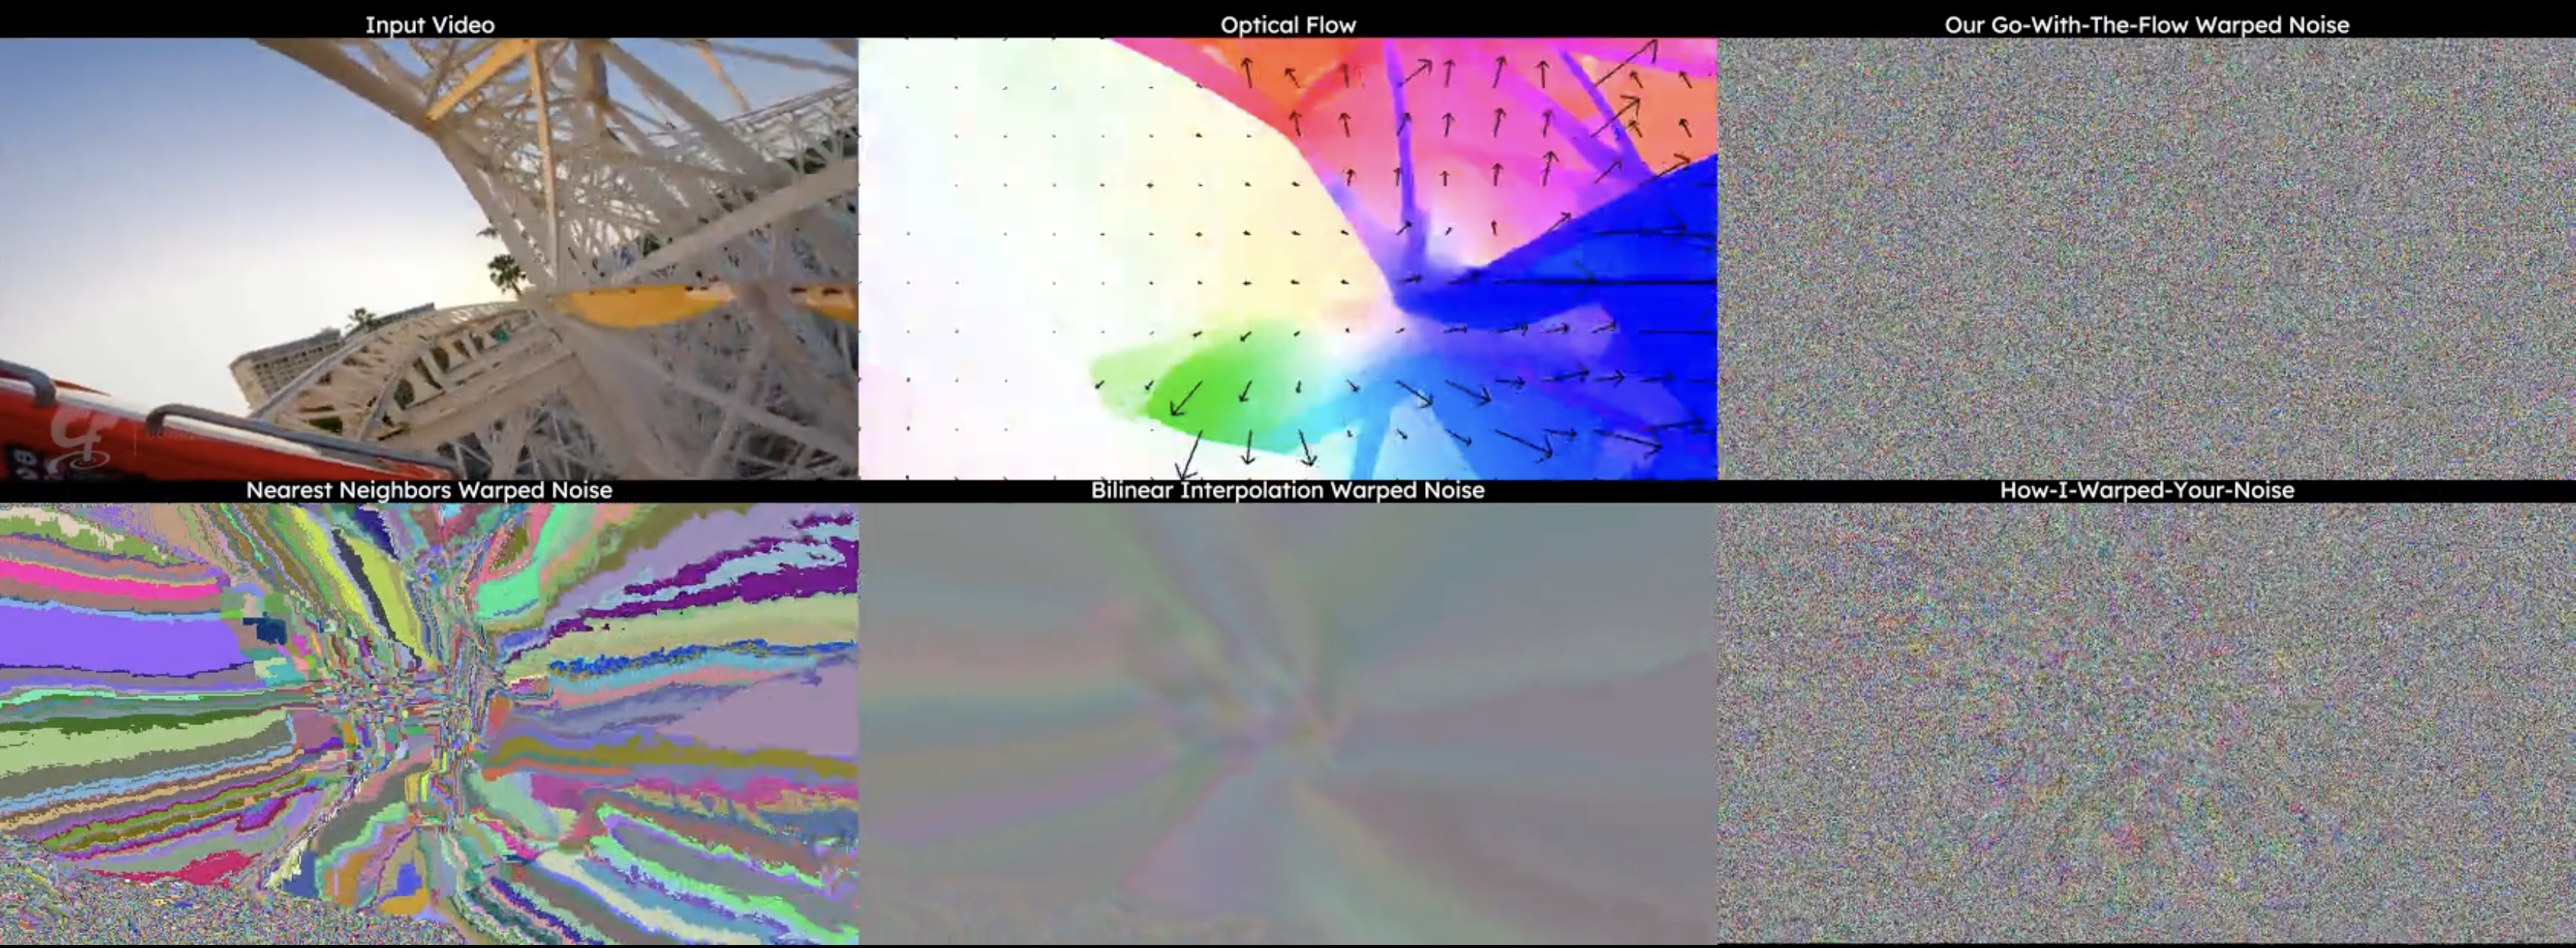
\includegraphics[width=1\linewidth]{fig/nongauss_vis.png}
    \caption{A direct visualization of the noise produced by our noise warping algorithm, HIWYN~\cite{chang2024warped}, bilinear, and nearest neighbor interpolations. The forward movement in this long roller-coaster video forces the noise to expand significantly. Early in the video, the HIWYN baseline produces visibly non-Gaussian results. See the full video on our \href{https://eyeline-research.github.io/Go-with-the-Flow/}{webpage}.}
    \label{fig:supp_warped_noise_flow_vis}
\end{figure*}

\begin{figure}
    \centering
    \includegraphics[width=1\linewidth]{fig/stroller_frame20.png}
    \caption{Using different noise warping algorithms on DeepFloyd~IF for video super-resolution on the DAVIS dataset.}
    \label{fig:supp_davis_deepfloyd}
\end{figure}

\begin{figure}
    \centering
    \includegraphics[width=1\linewidth]{fig/naz_diffrelight_grid11.jpg}
    \caption{Using different noise warping algorithms on DifFRelight for portrait video relighting. }
    \label{fig:supp_diffrelight_noisewarp}
\end{figure}


\section{The advantage of noise warping}

By using noise warping as a condition for motion, we effectively discard all structural information from our input video that cannot be inferred from motion alone. This can be advantageous, as demonstrated in \cref{fig:supp_windmill}. MotionClone does not use optical flow to guide the video trajectory, instead relying on manipulating activations within the diffusion model. As a result, the windmill gains an extra set of arms, whereas our method, which relies solely on motion information from optical flow via warped noise, does not introduce such artifacts.

\section{Comparison to the video diffusion base model without finetuning}

Interestingly, video diffusion models respond to noise warping even without training. In \cref{fig:supp_windmill} the rightmost column, even though the per-frame quality suffers, the flow of the output video still roughly follows the flow of the warped noise. However, because warped noise is statisically distinct from the pure Gaussian noise CogVideoX was trained on, without fine-tuning it can result in visual artifacts.

\section{User study settings and statistics}
\label{sec:supp_user_study}

\cref{fig:supp_user_study_screenshots_statistics} presents our user study questionnaires and statistics for two applications: (1) local object motion control, and (2) turnable camera movement video generation. Our questions focus on users' overall subjective preference, controllability, and temporal consistency.

\section{Model Agnostic}


Our method is data- and model-agnostic. It can be used to add motion control to arbitrary video diffusion models by only processing the noise sampling during fine-tuning. For example, it also works with AnimateDiff \cite{guo2024animatediff} fine-tuned on the WebVid dataset~\cite{Bain21} (the weights for this model on our \href{https://github.com/Eyeline-Research/Go-with-the-Flow}{GitHub} page). See its qualitative results in \cref{fig:supp_animatediff_grid}. Since release, the community has also trained a version of Go-with-the-Flow on HunyuanVideo (linked on our \href{https://github.com/Eyeline-Research/Go-with-the-Flow}{GitHub} page). Therefore, our method will generalize to future more advanced video diffusion base model.

\section{Pseudo code}

See \cref{listing:supp_algo_pseudo_code} for our noise warping pseudo code. See our source code and model checkpoints on \href{https://github.com/GoWithTheFlowPaper/gowiththeflowpaper.github.io}{GitHub}.

\begin{figure*}
    \centering
    \includegraphics[width=0.7\linewidth]{fig/windmills.pdf} 
    \caption{
    We show a \cutndrag~animation of a windmill rotating clockwise, next to the derived optical flow, our outputs, a baseline and an ablation. \textbf{Note} that the input video column appears to have two sets of panels because it's being cut and dragged over itself to create rotational motion. \textbf{When using noise warping is better}: Per-frame structural information can poison the result of MotionClone, giving the windmill an extra set of arms - whereas ours only receives motion information from optical flow alone via warped noise (there are no double-windmills in the optical flow patterns). \textbf{Ablation in rightmost column}: warped noise with $\deglevel=.5$ on the CogVideoX base model before we fine-tune it. Because warped noise is statisically distinct from the pure Gaussian noise CogVideoX was trained on, without fine-tuning it can result in visual artifacts. Note how although the per-frame quality suffers here, it still picks up on motion queues from the warped noise (the camera zooms into the windmill).}
    \label{fig:supp_windmill}
\end{figure*}

\begin{figure*}
    \centering
    \begin{subfigure}{.48\linewidth}
    \includegraphics[width=\linewidth]{fig/user_study_screenshot_1.png}
    \subcaption{User study interface and questions for local object motion control, corresponding to ~\cref{fig:comparisons_video_diffusion_object_motions} in the main paper.}
    \end{subfigure}
    \hfill
    \begin{subfigure}{.48\linewidth}
    \includegraphics[width=\linewidth]{fig/user_study_screenshot_2.png}
    \subcaption{User study interface and questions for turnable camera movement video generation, corresponding to ~\cref{fig:comparisons_video_diffusion_turning_object} in the main paper.}
    \end{subfigure}
    \\[12pt]
    \begin{subfigure}{0.48\linewidth}
    \centering
    \includegraphics[width=.7\linewidth]{fig/user_study_1_statistics_1.png}
    \subcaption{User study statistics for local object motion control on the first question ``\textit{Which video is the best overall?}''}
    \end{subfigure}
    \hfill
    \begin{subfigure}{0.48\linewidth}
    \centering
    \includegraphics[width=.7\linewidth]{fig/user_study_1_statistics_2.png}
    \subcaption{User study statistics for local object motion control on the second question ``\textit{Which video best aligns with the user intent for controlling the object movement based on the input?}''}
    \end{subfigure}
    \\[12pt]
    \begin{subfigure}{0.48\linewidth}
    \centering
    \includegraphics[width=.7\linewidth]{fig/user_study_1_statistics_1.png}
    \subcaption{User study statistics for local object motion control on the third question ``\textit{Which video best preserves the intended camera movement from the input?}''}
    \end{subfigure}
    \hfill
    \begin{subfigure}{0.48\linewidth}
    \centering
    \includegraphics[width=.7\linewidth]{fig/user_study_1_statistics_1.png}
    \subcaption{User study statistics for local object motion control on the fourth question ``\textit{Which video maintains the most consistent and stable motion throughout?}''}
    \end{subfigure}
    \\[12pt]
    \begin{subfigure}{0.48\linewidth}
    \centering
    \includegraphics[width=0.7\linewidth]{fig/user_study_2_statistics_1.png}
    \subcaption{User study statistics for motion transfer on the first question ``\textit{Which video has better overall quality?}''}
    \end{subfigure}
    \caption{User study questionnaires screenshots and statistics. For all the questions of both applications, our method (the rightmost bar plot) significantly wins the most user preferences.}
    \label{fig:supp_user_study_screenshots_statistics}
\end{figure*}

% \begin{figure*}
%     \centering
%     \includegraphics[width=1\linewidth]{fig/animatediff.jpg}
%     \caption{Fine-tuning AnimateDiff with our warped noise flow. All rows share the same movements, and all columns share the same text prompts. The first column is the reference video providing the flow to warp the noise in column 2, which is then used to diffuse all videos to the right. Please zoom in to see the captions for each row (input videos driving movement and warping noise via optical flow) and each column (text prompt for each video cell). Refer to our project video to see these in animation form.}
%     \label{fig:supp_animatediff_grid}
% \end{figure*}

\begin{figure*}
    \centering
    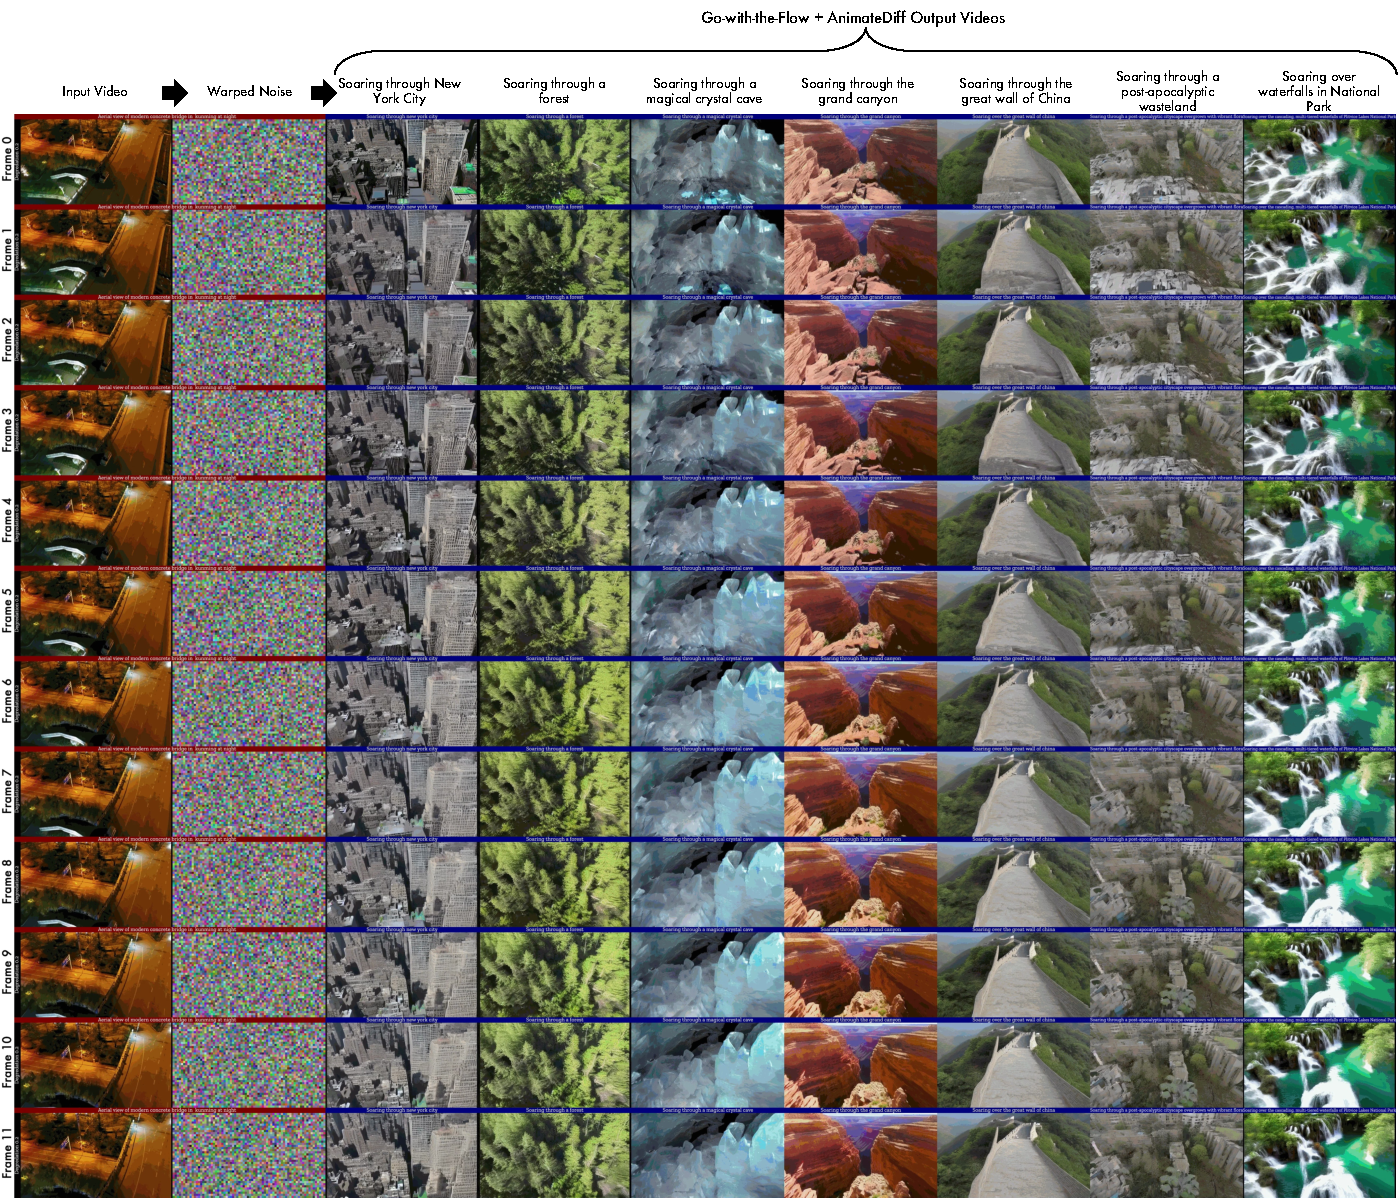
\includegraphics[width=1\linewidth]{fig/AnimateDiffAnimation.pdf}
    \caption{Fine-tuning AnimateDiff with our warped noise flow. We used Go-with-the-Flow to fine-tune AnimateDiff T2V, and display the results above. The input video is on the left, and from that video we derive warped noise which is used to initialize AnimateDiff on the columns to its right with different text prompts.}
    \label{fig:supp_animatediff_grid}
\end{figure*}

\begin{figure*}
\begin{lstlisting}
def warp_noise(prev_frame, cur_frame, prev_noise, prev_weight):

    height, width, _ = prev_frame.shape

    flow = optical_flow(prev_frame, cur_frame) # Agnostic to the optical flow algorithm
    backwards_flow = -flow # A cheap approximation of optical_flow(cur_frame, prev_frame)

    expansion_noise    = zeros(height, width)
    contraction_noise  = prev_noise.copy()

    expansion_mask     = ones (height, width, type=bool)
    contraction_mask   = zeros(height, width, type=bool)

    for x in range(width): for y in range(height):
        dx, dy = flow[x,y]
        if 0 <= x+dx <= width-1 and 0 <= y+dy <= height-1:
            # This particle stays in bounds
            expansion_mask  [x+dx, y+dx] = False
            contraction_mask[x   , y   ] = True  # Contraction mask is True where 

    for x in range(width): for y in range(height):
        if expansion_mask[x, y]:
            dx, dy = backwards_flow[x,y]
            expansion_noise [x, y] = prev_noise[x+dx, y+dy]

    # We've decided which source pixels are involved in contraction and expansion now
    contraction_noise &= contraction_mask
    expansion_noise, contraction_noise, cur_weight = jointly_regaussianize_and_rebalance_weights(
        expansion_noise, contraction_noise, prev_weight
    ) # Regaussianize all noise values here, and divide the weights by the number of pixels in each bin

    contraction_weight = zeros(height, width)
    for x in range(width): for y in range(height):
        if contraction_mask[x, y]:
            # Contraction treats the noise pixels as particles, each moving from the source to the
            # destination with this flow
            dx, dy = flow[x,y]
            # Contraction is a weighted sum of source pixels to a destination pixel
            pixel_weight = cur_weight[x, y]
            # Sum all the source noise pixels that contract to the same destination
            contraction_noise [x+dx, y+dy] += prev_noise[x, y] * pixel_weight
            # When we multiply a noise pixel by a weight, the variance changes by that weight squared
            contraction_weight[x+dx, y+dy] += pixel_weight ** 2 
    contraction_noise /= sqrt(contraction_weight) # Adjust the variance of the summed contracted noise

    # Mixing contraction and expansion noises with their respective masks
    cur_noise = contraction_noise & contraction_mask + expansion_noise & expansion_mask

    return cur_noise, cur_weight
\end{lstlisting}
\caption{Our noise warping pseudo code.}
\label{listing:supp_algo_pseudo_code}
\end{figure*}


\end{document}
